\documentclass[crop,tikz]{standalone}
\usepackage[subpreambles=true]{standalone}

../presentation_7_30_18/preamble.tex

\begin{document}

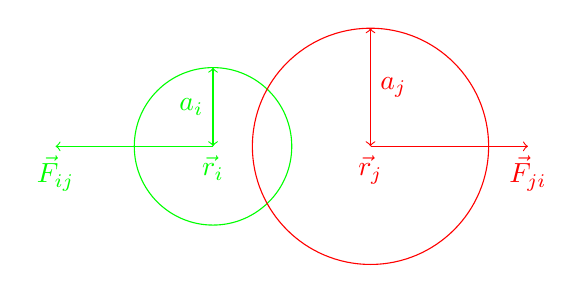
\begin{tikzpicture}[scale=1]
\draw[green] (0, 0) circle (1) node[below]{$\vec{r}_i$};
\draw[<->, green] (0, 0) -- (0, 1) node[midway, left]{$a_i$};
\draw[->, green] (0, 0) -- (-2, 0) node[left, below]{$\vec{F}_{ij}$};
\draw[red] (2, 0) circle (1.5) node[below]{$\vec{r}_j$};
\draw[<->, red] (2, 0) -- (2, 1.5) node[midway, right]{$a_j$};
\draw[->, red] (2, 0) -- (4, 0) node[right, below]{$\vec{F}_{ji}$};
\end{tikzpicture}

\end{document}
